\section{Tema 4: Conservación de la cantidad de movimiento}
\subsection{Teorema del transporte de Reynolds para la cantidad de movimiento}
Sea un volumen sometido a un conjunto de fuerzas:
\begin{figure}[H]
	\centering
	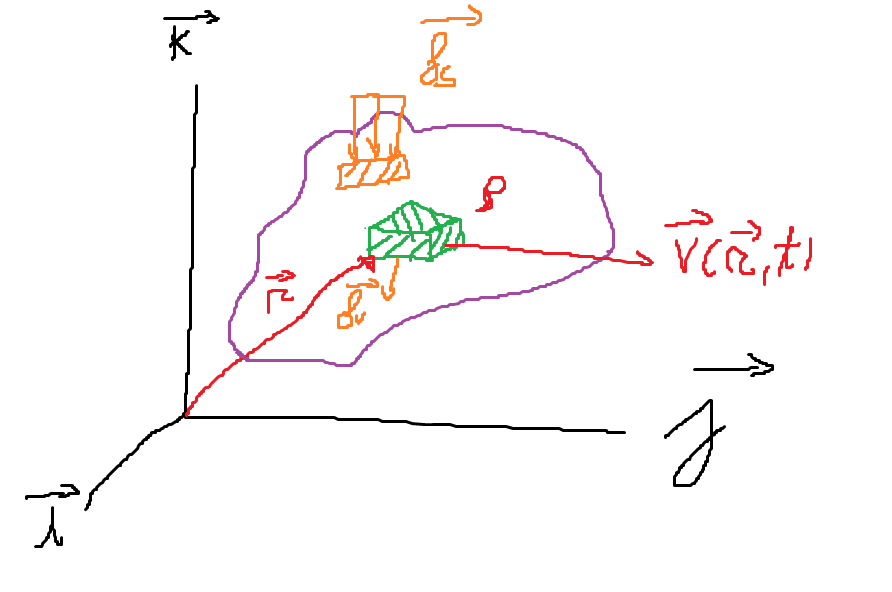
\includegraphics[width=0.7\linewidth]{imagenesTema4/magnitudesFuerzas}
	\caption{Magnitudes principales que influencian la cantidad de movimiento.}
	\label{fig:magnitudesfuerzas}
\end{figure}

Aplicando al teorema del transporte de Reynolds la función $\Phi=\rho\vec{v}$ y una similitud con la segunda ley de Newton se obtiene para volúmenes fluidos:
\[\iiint_{V_f}\vec{f}_V\,dV+\oiint_{S_f}\vec{f}_s\,dS=
\frac{d}{dt}\iiint_{V_f}\rho\vec{v}\,dV=
\iiint_{V_f}\frac{\partial \rho\vec{v}}{\partial t}\,dV+\oiint_{S_f}\rho\vec{v}\left(\vec{v}\cdot\vec{n}\right)\,dS\]

Para un volumen de control:
\[\iiint_{V_f}\vec{f}_V\,dV+\oiint_{S_f}\vec{f}_s\,dS=
\frac{d}{dt}\iiint_{V_f}\rho\vec{v}\,dV=
\iiint_{V_c}\frac{\partial \rho\vec{v}}{\partial t}\,dV
+\oiint_{S_c}\rho\vec{v}\left[\left(\vec{v}-\vec{v}_c\right)\cdot\vec{n}\right]\,dS\]

En estas expresiones aparecen dos tipos de fuerzas:
\begin{enumerate}
	\item Fuerzas volumétricas $\vec{f}_v$
	\item Fuerzas superficiales $\vec{f}_s$
\end{enumerate}
\subsection{Ecuaciones de Navier-Stokes}

\subsection{Número de Reynolds}

\subsection{Teorema de Bernouilli}
